\documentclass[10pt]{beamer}

\definecolor{dlightblue}{rgb}{0.65,0.65,0.98}
\definecolor{lightblue}{rgb}{0.85,0.85,1.0}
\definecolor{llightblue}{rgb}{0.95,0.95,0.98}
\definecolor{darkblue}{rgb}{0,0,.6}
\definecolor{darkred}{rgb}{.6,0,0}
\definecolor{darkgreen}{rgb}{0,.6,0}
\definecolor{darkbrown}{rgb}{0.5,0.30,0.10}
\definecolor{red}{rgb}{.98,0,0}

\definecolor{refcolor}{rgb}{0.0,0.6,0.0}
\setbeamercolor{upcol}{fg=black,bg=lightblue}
\setbeamercolor{lowcol}{fg=black,bg=llightblue}
\newenvironment{colorblock}
{\begin{beamerboxesrounded}[upper=upcol,lower=lowcol,shadow=false]}
{\end{beamerboxesrounded}}

\setbeamercolor{alertupcol}{fg=black,bg=dlightblue}
\setbeamercolor{alertlowcol}{fg=black,bg=lightblue}
\newenvironment{alertcolorblock}
{\begin{beamerboxesrounded}[upper=alertupcol,lower=alertlowcol,shadow=false]}
{\end{beamerboxesrounded}}
\setbeamercolor{block body}{bg=llightblue}
\setbeamercolor{block title}{fg=black,bg=lightblue}
\setbeamercovered{transparent}

\title{Reminder: Preprocessing of the Trajectory Data}
\author[Tobias Stollenwerk]
{\emph{Tobias Stollenwerk}\inst{1},
Bryan O'Gorman\inst{2},
Salvatore Mandr\`{a}\inst{2},
Davide Venturelli\inst{2},
Eleanor G. Rieffel\inst{2}\\
}
\institute[NASA and DLR]
{\inst{1}
German Aerospace Center (DLR) \\
\inst{2}
NASA QuAIL \\
}
\date{Dec 20, 2016}
\usetheme{dlr}
\begin{document}

\begin{frame}
    \titlepage
\end{frame}

\begin{frame}[t]{Wind-Optimal Trajectories}
    \begin{itemize}
        \item 984 transatlantic flights on a single day
    \end{itemize}
    \begin{center}
        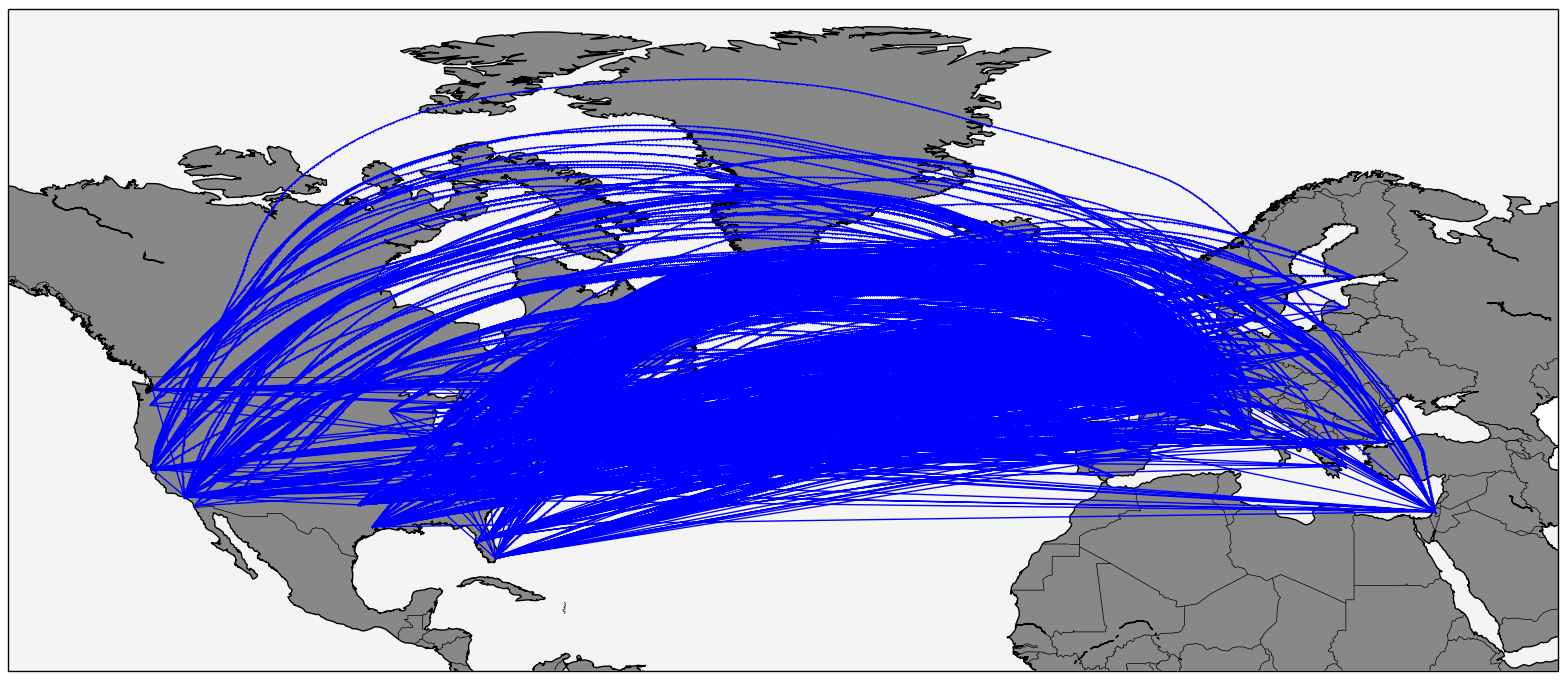
\includegraphics[width=1.0\textwidth]{images/wind_optimal_trajectories.png}
    \end{center}
    \vspace{-0.6cm}
    \hfill \tiny{Data from O. Rodionova}
\end{frame}
\begin{frame}[t]{Optimization Problem Formulation}
    \begin{block}{Variables}
        \begin{itemize}
            \item Departure delays $d_i$ for each flight $i$
                \hspace{1cm}
                \begin{minipage}{0.3\linewidth}
                    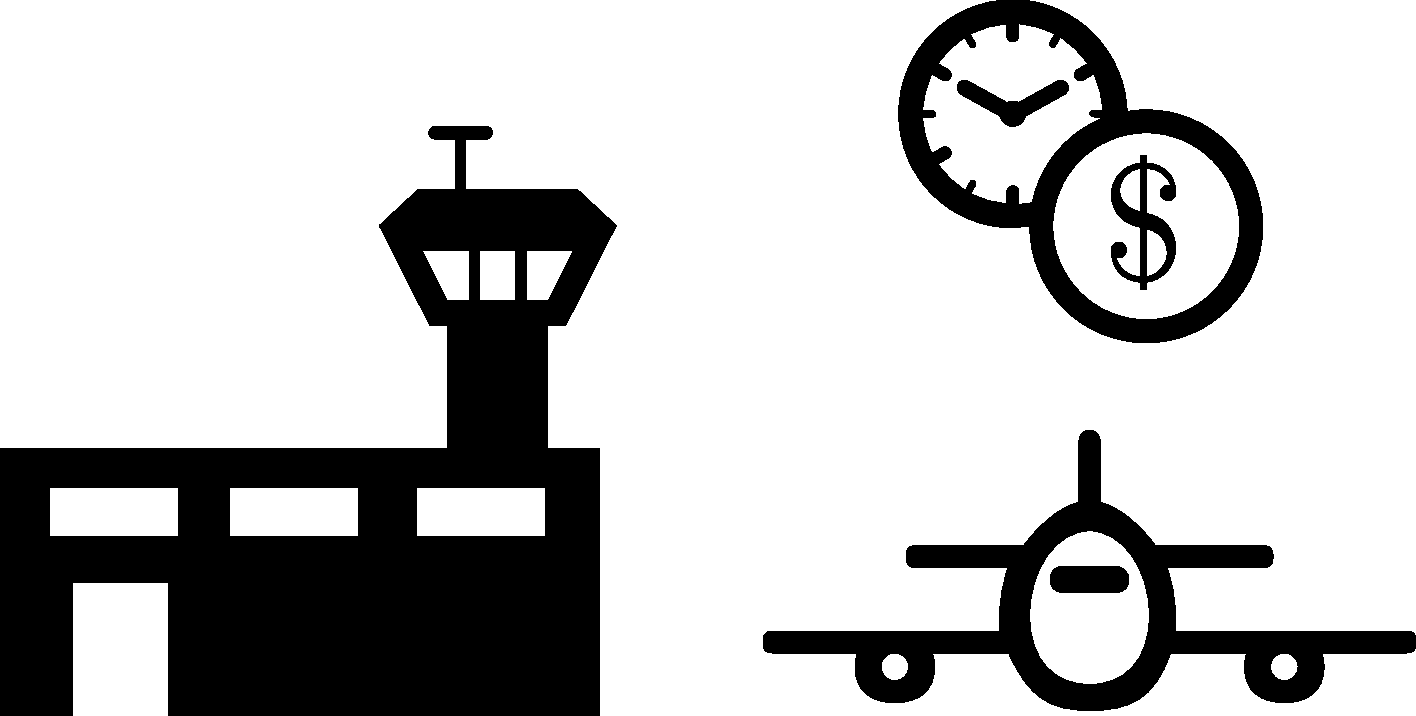
\includegraphics[width=0.8\textwidth]{images/departure_delay.pdf} \\
                \end{minipage}
            \item 
                \begin{minipage}[t]{0.5\linewidth}
                    Maneuver of flight $i$ to avoid conflict $k$ introduce delay $d_{ik}$
                \end{minipage}
                \hspace{1cm}
                \begin{minipage}[c]{0.3\linewidth}
                    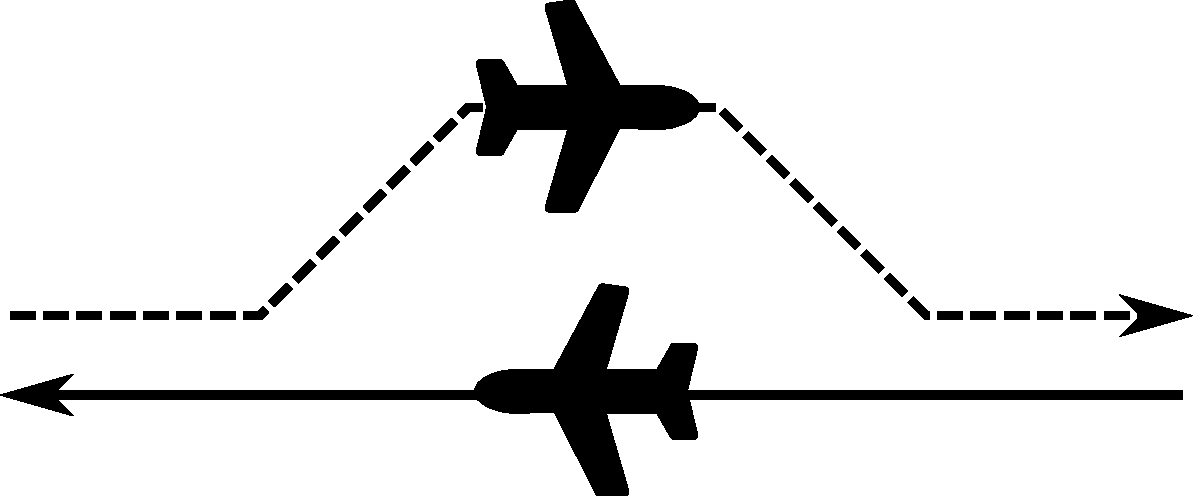
\includegraphics[width=0.9\textwidth]{images/conflict_avoiding_maneuver.pdf}
                \end{minipage}
       \end{itemize} 
    \end{block}
    \begin{block}{Cost function contribution}
        \centering
        Total delay: 
        $
            C = \sum_i d_i + \sum_{ik} d_{ik}
        $
    \end{block}
\end{frame}
 
\begin{frame}[t]{Optimization Problem Formulation - Simplifications}
    \begin{itemize}
        \item Only pairwise conflicts 
            \hfill
            \begin{minipage}[c]{0.6\linewidth}
                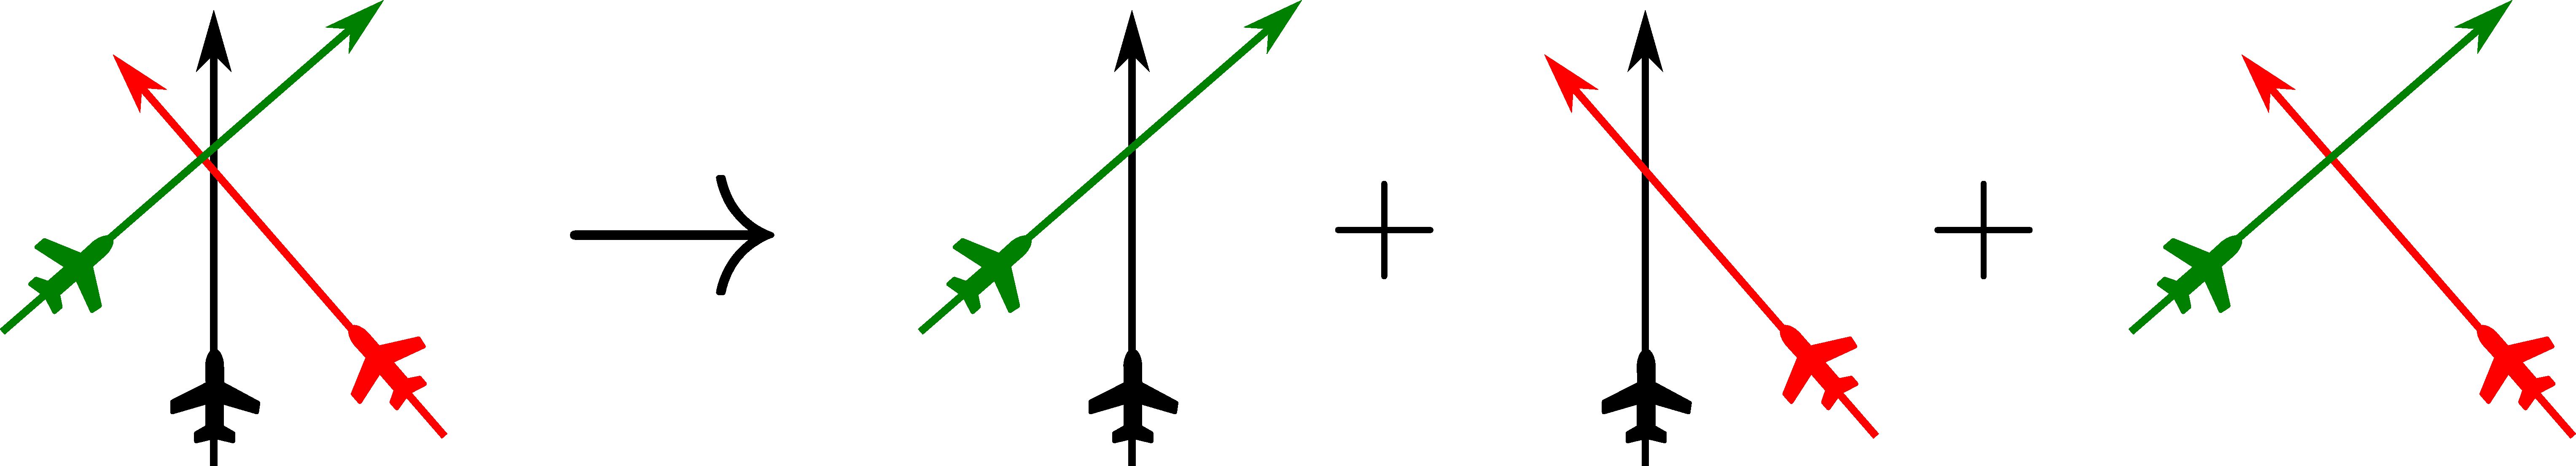
\includegraphics[width=0.9\textwidth]{images/pairwise_conflicts.pdf}
            \end{minipage}
            %\\
            %$\Rightarrow$ Each conflict $k$ is attached to exacly two flights $i_k$ $j_k$
        \item Conflict avoiding maneuvers impact {\bf only} on delay.
            \hfill
            \begin{minipage}[c]{0.3\linewidth}
                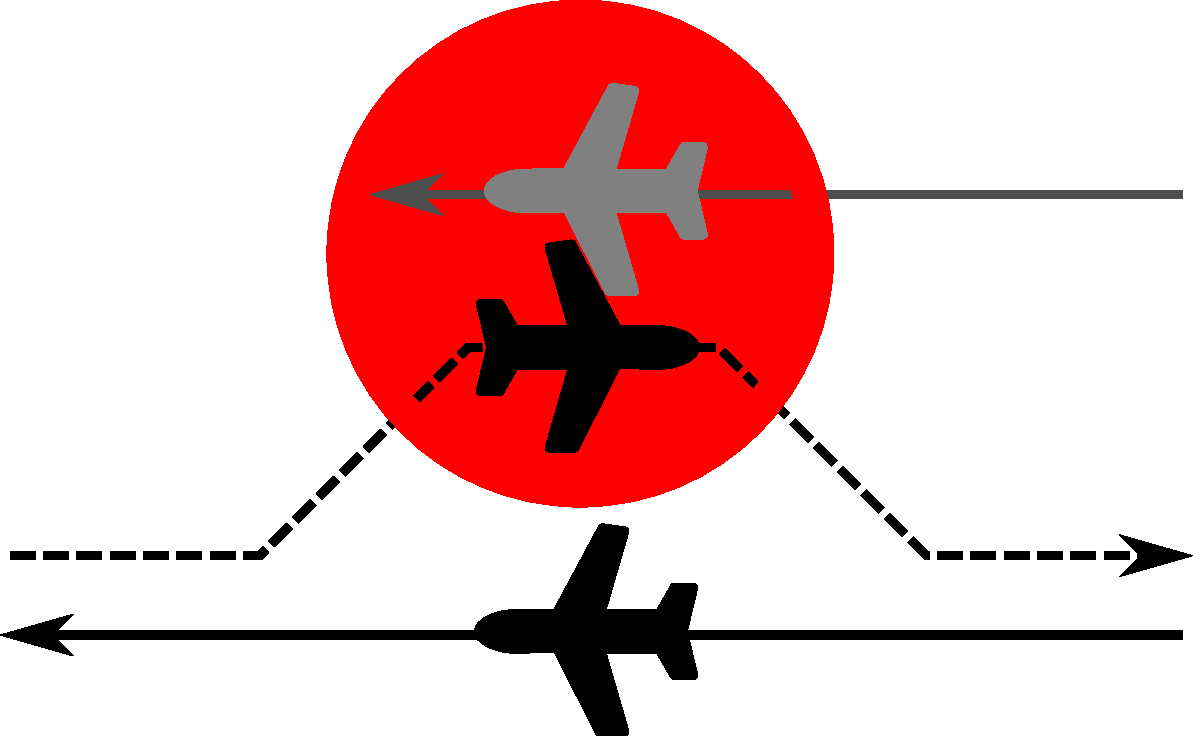
\includegraphics[width=0.9\textwidth]{images/conflict_avoiding_maneuver_pairwise_overlay1.pdf}
            \end{minipage}
    \end{itemize} 
\end{frame}
\begin{frame}[t]{Conflict Avoidance - Arrival Times}
    \begin{itemize}
        \item Difference of arrival times at the conflict between flights $i$ and $j$,  $\Delta_k = T_{ik} - T_{jk}$ \\
            \hspace{0.5cm}

            \begin{minipage}[c]{0.9\linewidth}
                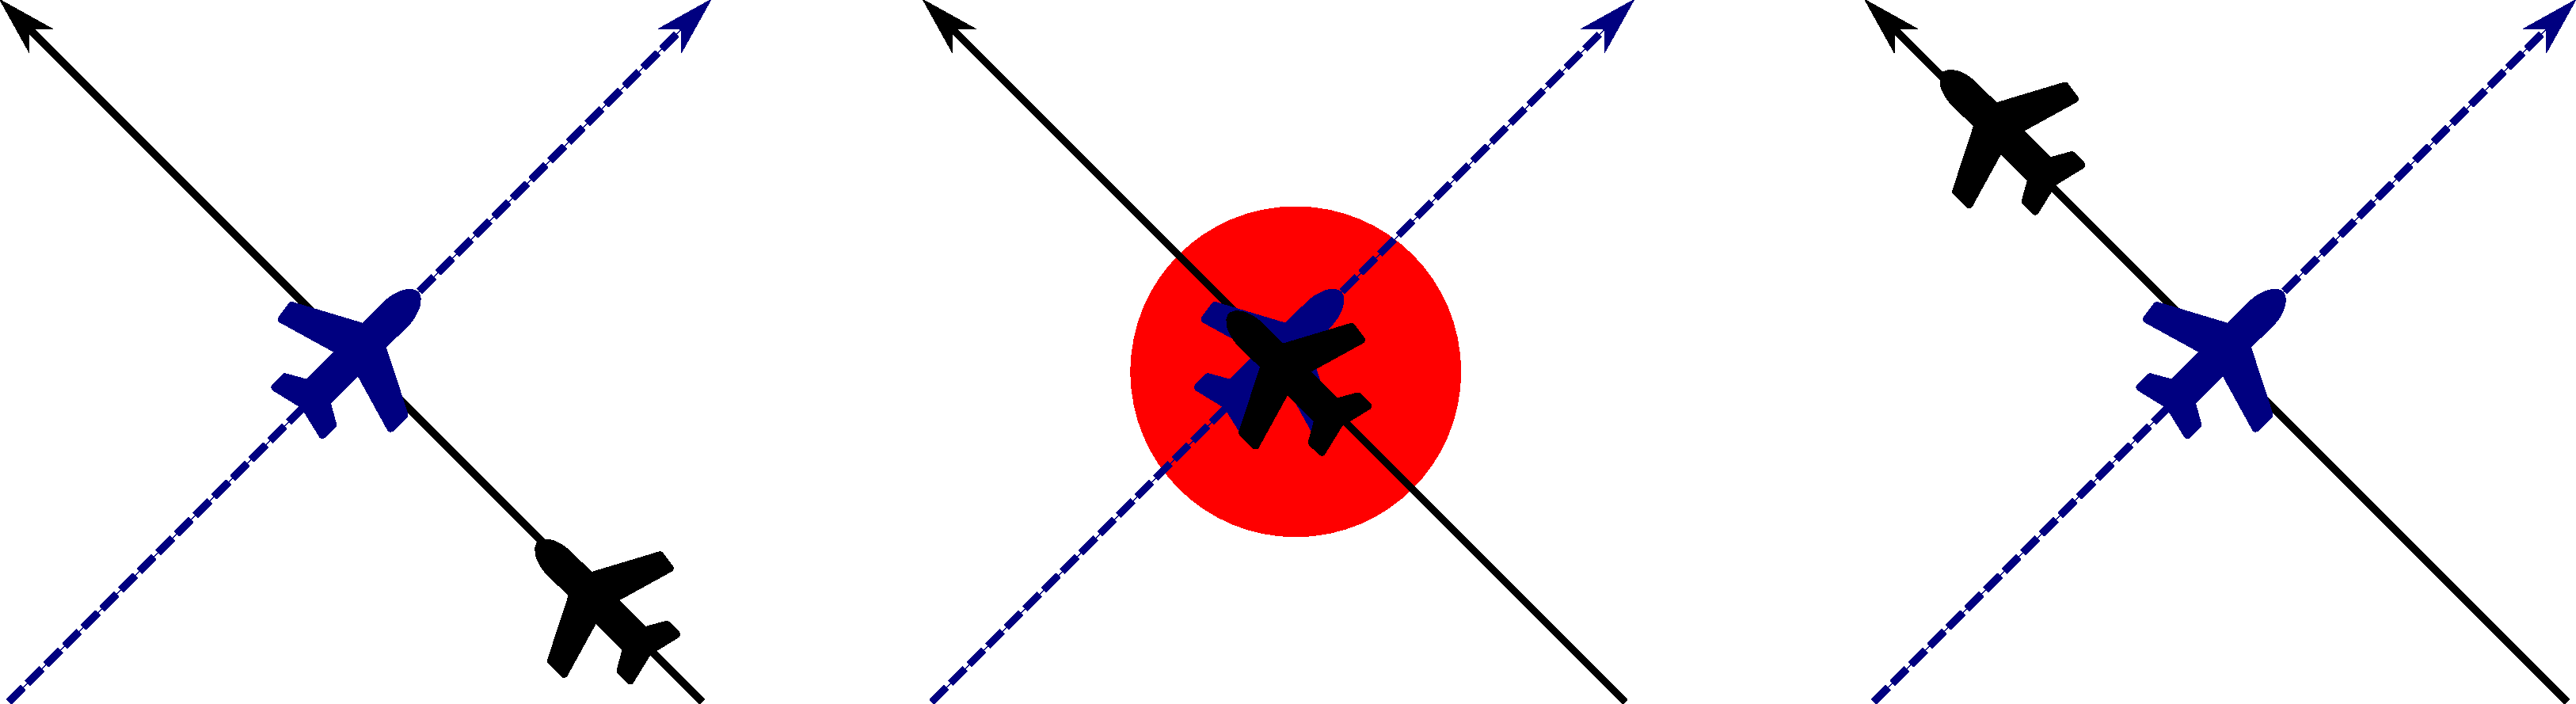
\includegraphics[width=1.0\textwidth]{images/conflict_avoiding_arrival_times.pdf}
                \\ 
            \end{minipage}
            \hspace{0.5cm}
            \\
            $\qquad \Delta_k \ll 0$
            $\qquad \qquad \qquad \Delta_k \approx 0$
            $\quad \qquad \qquad \qquad \Delta_k \gg 0$
        \item Delay resulting from conflict avoidance is function of $\Delta_k = T_{ik} - T_{jk}$:
            \begin{equation*}
                d_{ik} = \mathcal{D}_{ik}(\Delta_k)
            \end{equation*}
            \hfill 
            \begin{minipage}[c]{0.3\linewidth}
                \vspace{-1cm}
                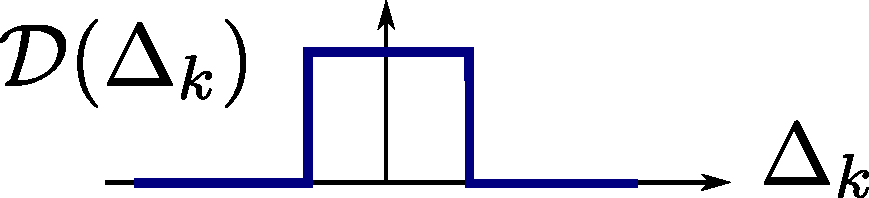
\includegraphics[width=1.0\textwidth]{images/conflict_delay_function.pdf}
            \end{minipage}
    \end{itemize} 
\end{frame}
\begin{frame}[t]{Conflict Avoidance - Maneuver Parameter}
    \begin{itemize}
        \item Maneuver parameter $a_k$, e.g. $a_k \in [0, 1]$
            \hfill
            \begin{minipage}[c]{0.9\linewidth}
                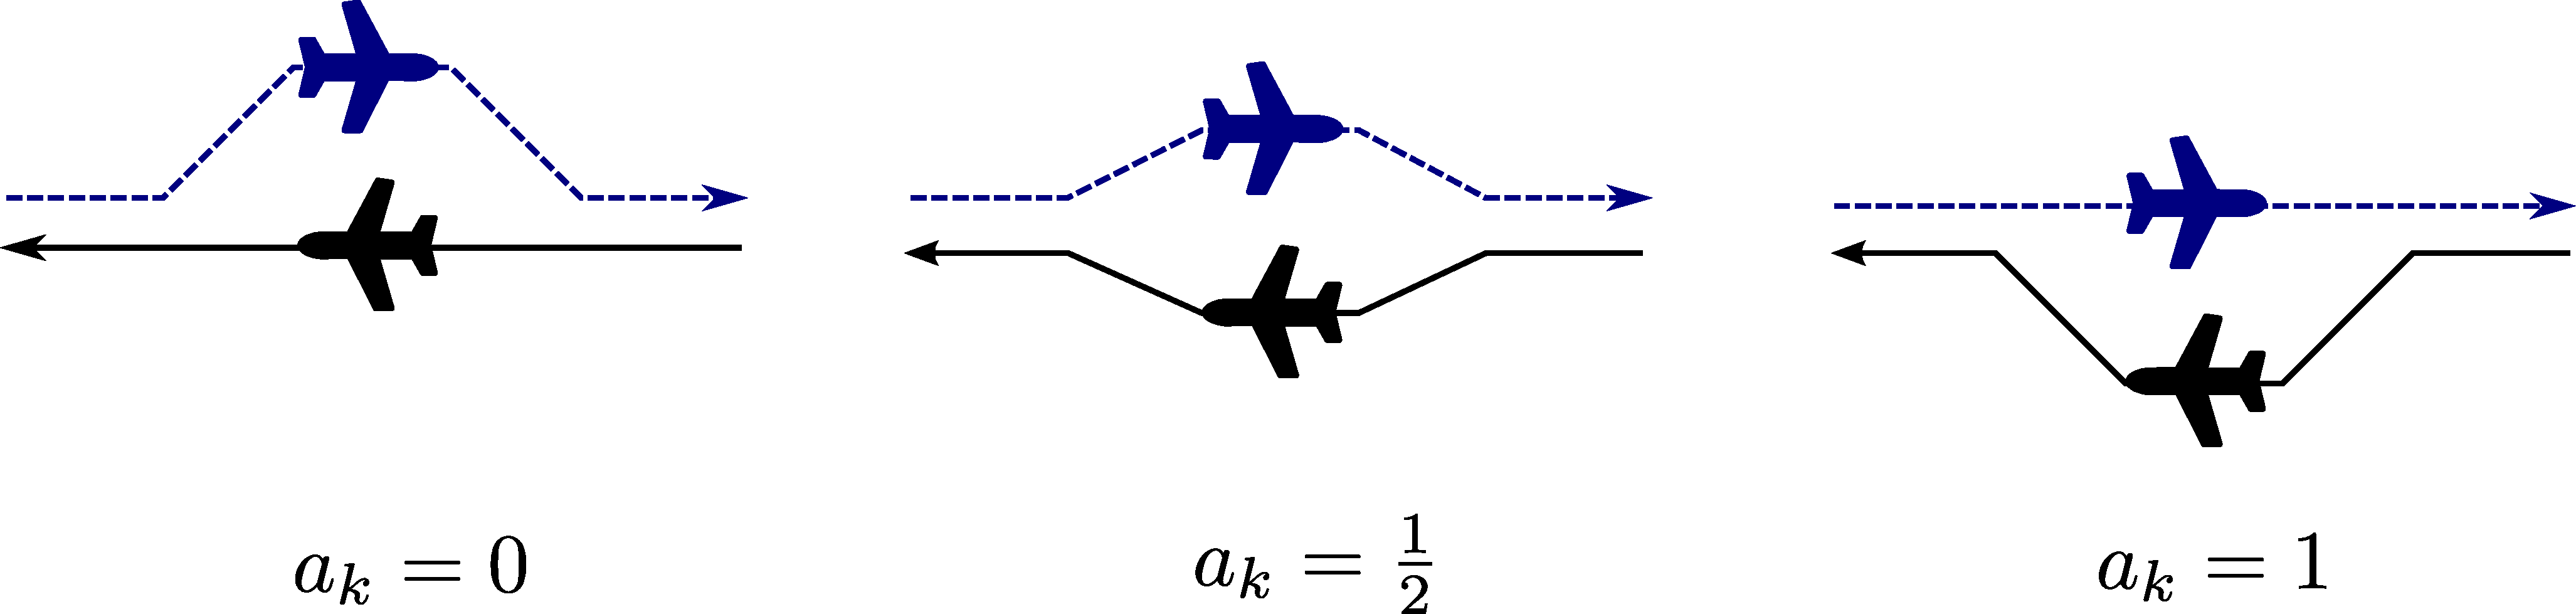
\includegraphics[width=1.0\textwidth]{images/conflict_avoiding_maneuver_parameter.pdf}
            \end{minipage}
        \item Delay resulting from conflict avoidance depends on maneuver:
            \begin{equation*}
                d_{ik} = \mathcal{D}_{ik}(\Delta_k, a_k) 
            \end{equation*}
    \end{itemize} 
    \begin{center}
    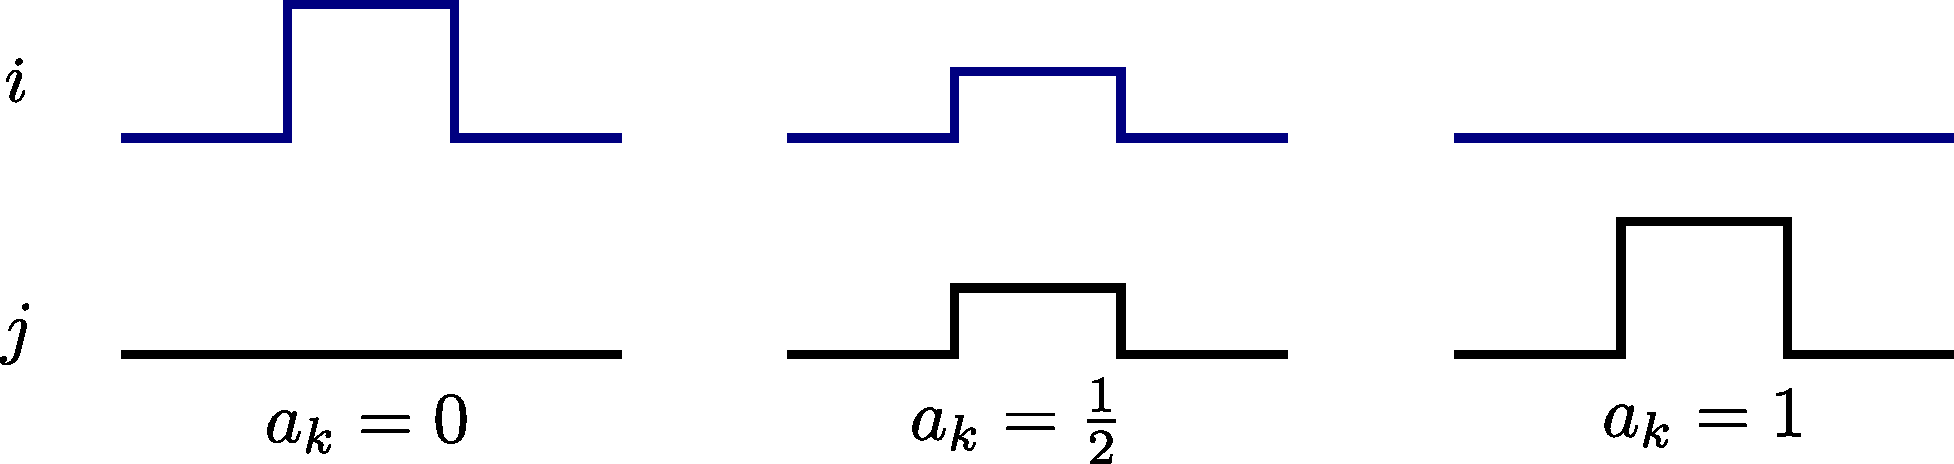
\includegraphics[width=0.76\textwidth]{images/conflict_delay_function_maneuver.pdf}
    \end{center}

\end{frame}


\begin{frame}[t]{Optimization Problem Formulation}
    \begin{itemize}
        \item Arrival time of flight $i$ at conflict $k$ is delayed by preceding conflicts
            \begin{equation*}
                T_{ik} = t_{ik} + d_i +  \sum_{p<k} d_{ip} \qquad t_{ik} \text{: Wind-optimal arrival time}
            \end{equation*}
        \item Optimization problem 
            \begin{equation*}
                \underset{d_i, d_{ik}, a_k}{\text{minimize}} \; \sum_i d_i + \sum_{ik} \mathcal{D}_{ik}(\Delta_{k}, a_k)
            \end{equation*}
            \begin{align*}
                \text{subject to} \qquad
                & \Delta_{k} = t_{ik} + d_i + \sum_{p<k} d_{ip} - t_{jk} - d_j - \sum_{q<k} d_{jq} \\
                & d_{ik} = \mathcal{D}_{ik}(\Delta_{k}, a_k) 
            \end{align*}

    \end{itemize}
\end{frame}
\begin{frame}[t]{Simplification: Delay-Only Model}
    \begin{block}{Optimization problem}
            \begin{equation*}
                \underset{d_i}{\text{minimize}} \; \sum_i d_i 
            \end{equation*}
            \begin{align*}
                \text{subject to} \qquad
                | t_{ik} + d_i - t_{jk} - d_j
 | < 3 \text{ minutes} \quad \forall k\\ 
            \end{align*}
    \end{block}
\end{frame}
\begin{frame}[t]{Precalculating Conflicts}
    \begin{minipage}[t]{0.4\linewidth}
        Given the trajectories of all flights $i$ 
    \end{minipage}
    \hfill
    \begin{minipage}[c]{0.5\linewidth}
        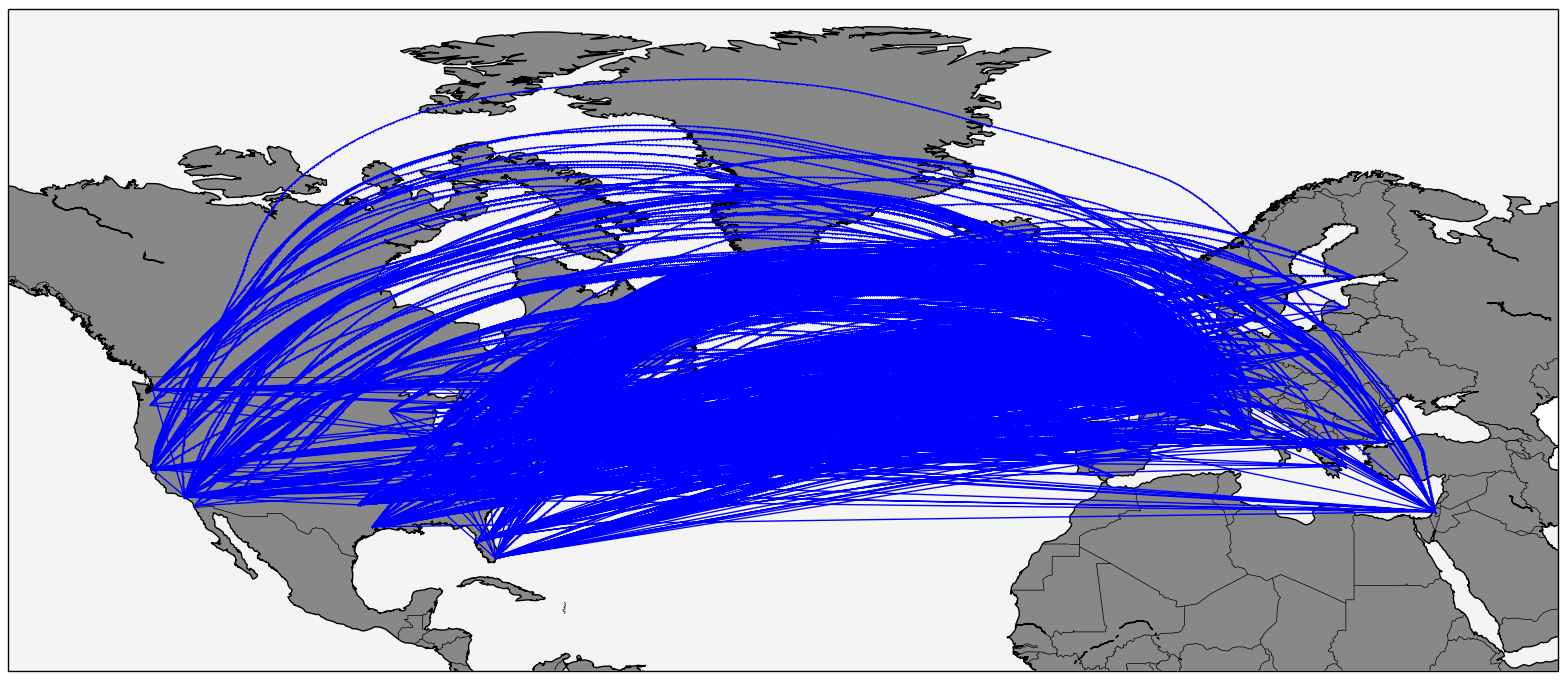
\includegraphics[width=1.0\textwidth]{images/wind_optimal_trajectories.png}
    \end{minipage}
    \vspace{1cm}
    \begin{center}
        $\Rightarrow$ How to calculate the \emph{potential} conflicts $k$?
    \end{center}
\end{frame}
%\begin{frame}[c]{}
    %\begin{center}
        %\hspace{-1cm}
        %{\LARGE Conflict Calculation}
    %\end{center}
%\end{frame}
\begin{frame}[t]{Spatial Conflict Detection}
    \begin{itemize}
        \item Spatial conflict, if trajectory points are close (30 NM) to each other.
    \end{itemize}
    \begin{overprint}%
	\begin{columns}[t]
        \visible<1-> {%
		\column{0.45\textwidth}
            \begin{block}{Brute force algorithm}
                \begin{itemize}
                    \item Check distance between nearly {\bf all} trajectory points
                \end{itemize} 
                \begin{center}
                    \only<1>{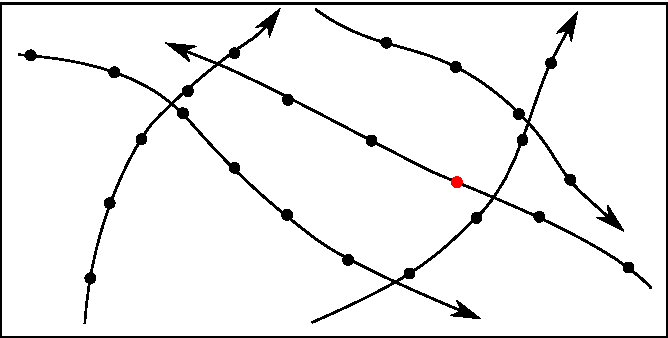
\includegraphics[width=1.0\textwidth]{images/spatial_conflict_detection_00.pdf}}
                    \only<2,3,4>{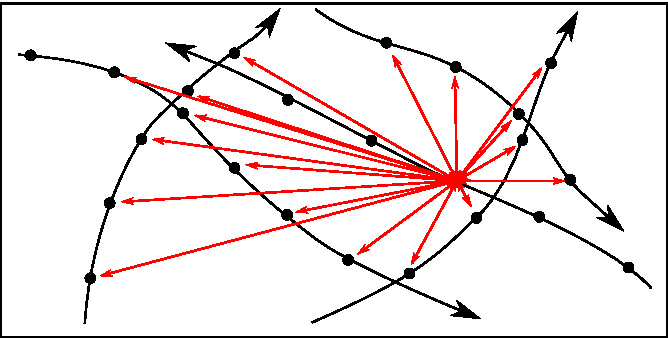
\includegraphics[width=1.0\textwidth]{images/spatial_conflict_detection_01.pdf}}
                \end{center}
            \end{block}
        }%
        \visible<3-> {%
		\column{0.45\textwidth}
            \begin{block}{Coarse grid algorithm}
                \begin{itemize}
                    \item Map trajectory points to coarse grid
                \end{itemize} 
                \begin{center}
                    \only<3>{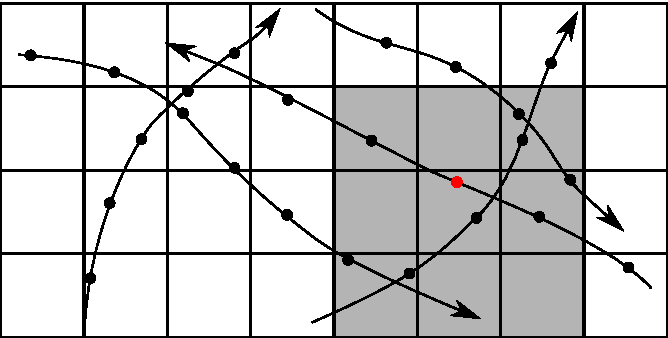
\includegraphics[width=1.0\textwidth]{images/spatial_conflict_detection_02.pdf}}
                    \only<4>{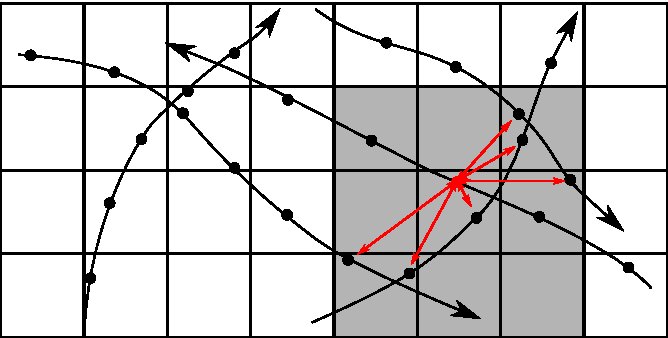
\includegraphics[width=1.0\textwidth]{images/spatial_conflict_detection_03.pdf}}
                \end{center}
                \visible<4> {
                \vspace{-0.3cm}
                \begin{itemize}
                    \item Check distance only with neighboring cells
                \end{itemize} 
                }
            \end{block}
        }%
    \end{columns}
    \end{overprint}%
\end{frame}
\begin{frame}[t]{Potential Conflicts}
    \begin{itemize}
        \item Potential conflict: Spatial conflict which can become real conflict
            \hspace{0.5cm}

            \begin{minipage}[c]{0.9\linewidth}
                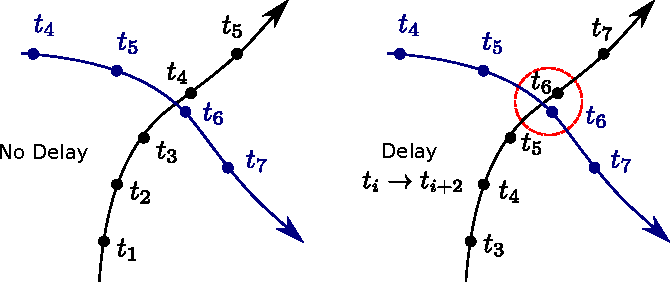
\includegraphics[width=1.0\textwidth]{images/potential_conflict.pdf}
                \\ 
            \end{minipage}
            \\
            \hspace{1.0cm}
            Spatial Conflict
            \hspace{3cm}
            Real Conflict
        \item First step: Potential conflict, if difference in wind-optimal arrival times $t_{ik}-t_{jk} < 2 $ hours.
    \end{itemize} 
\end{frame}

\begin{frame}[t]{Potential Conflicts}
    \begin{itemize}
        \item How to reduce the huge number of potential conflicts: $6,609,623$?
    \end{itemize}
    \vspace{-0.2cm}
    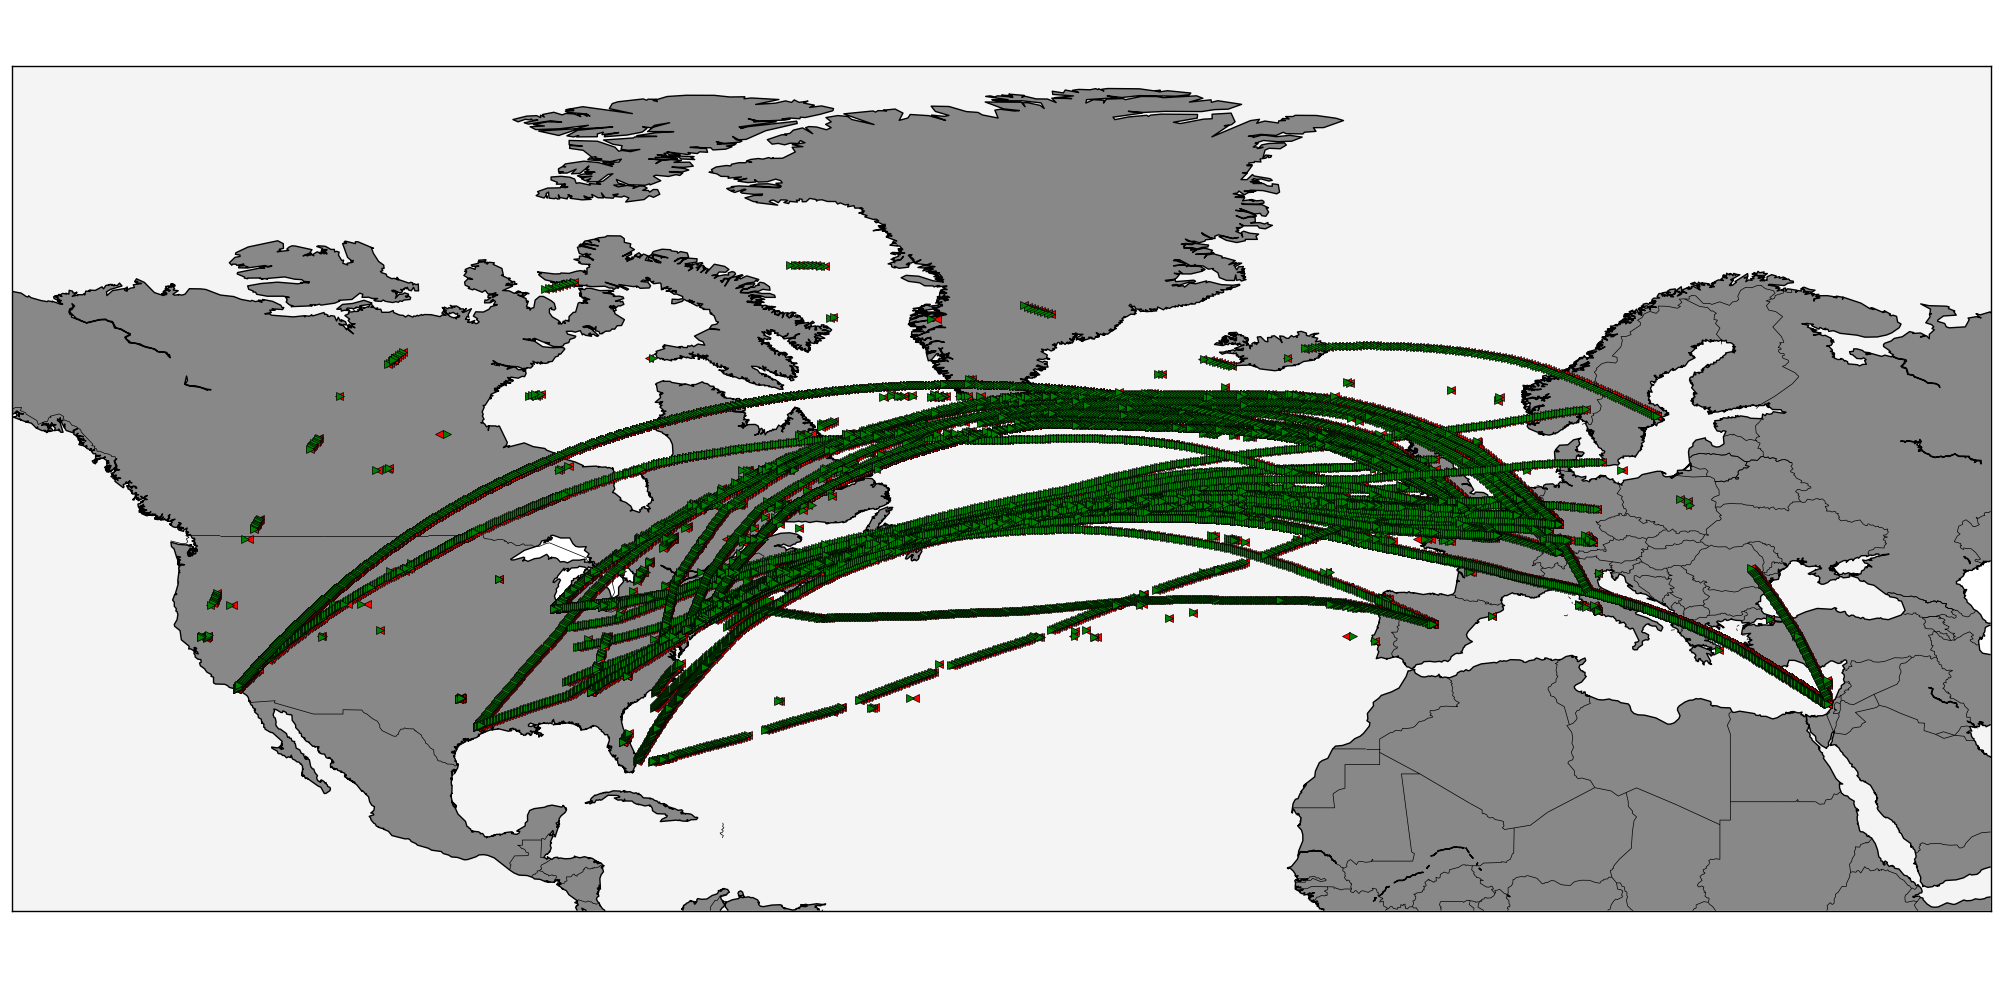
\includegraphics[width=1.0\textwidth]{images/spatial_conflicts_data.png}
\end{frame}
\begin{frame}[t]{Potential Conflicts - Classification}
    Reduce the vast number of potential conflicts by categorizing:
    \begin{itemize}
        \item Point Conflict: Isolated in time $N_\text{point} = 265$
        \item Parallel conflict: Point conflicts consecutive in time $N_\text{parallel} = 20867$
        \item Reduction of $99.7 \%$
    \end{itemize}
    \begin{center}
        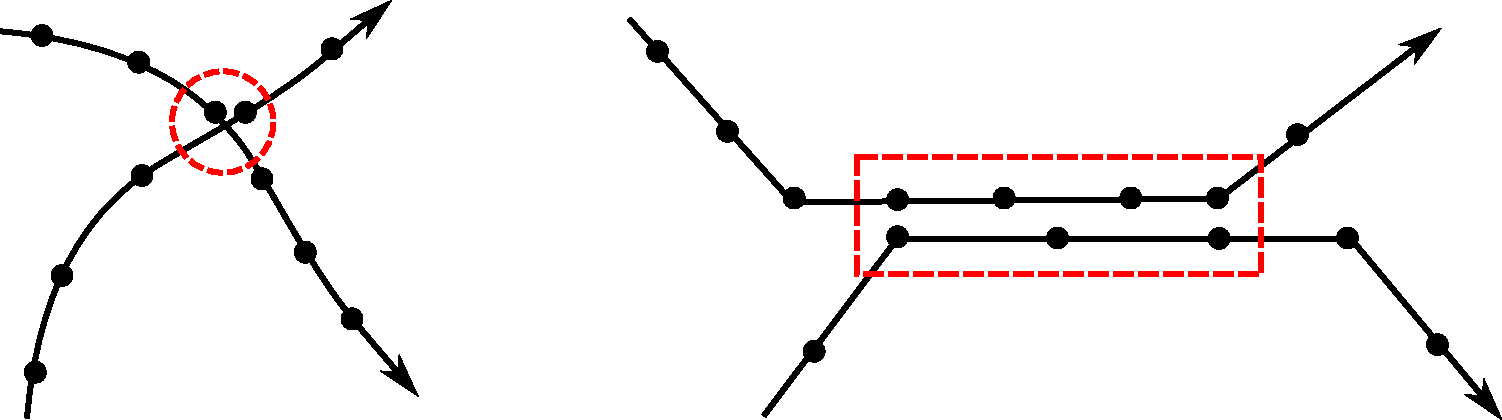
\includegraphics[width=0.9\textwidth]{images/spatial_conflict_categories.pdf}
    \end{center}
    \hspace{1.0cm}
    Point Conflict
    \hspace{3.5cm}
    Parallel Conflict
\end{frame}
\begin{frame}[t]{Potential Conflicts - Reduction}
    Self-consistent algorithm:
    \begin{itemize}
        \item For each flight, order conflicts in time
        \item For each potential conflict, calculate the maximal delay of both flights
        \item Remove potential conflicts which can not become real conflicts
        \item Repeat the above steps until convergence ($N_\text{spatial}$ invariant) 
    \end{itemize}
    \begin{center}
        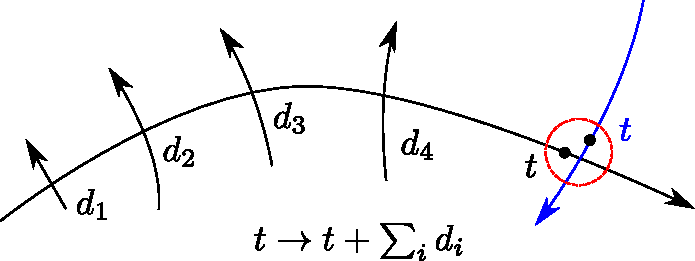
\includegraphics[width=0.8\textwidth]{images/potential_conflict_detection.pdf}
    \end{center}
\end{frame}
\begin{frame}[t]{Potential Conflicts - Reduction}
    \begin{center}
        %\hspace{-1.5cm}
        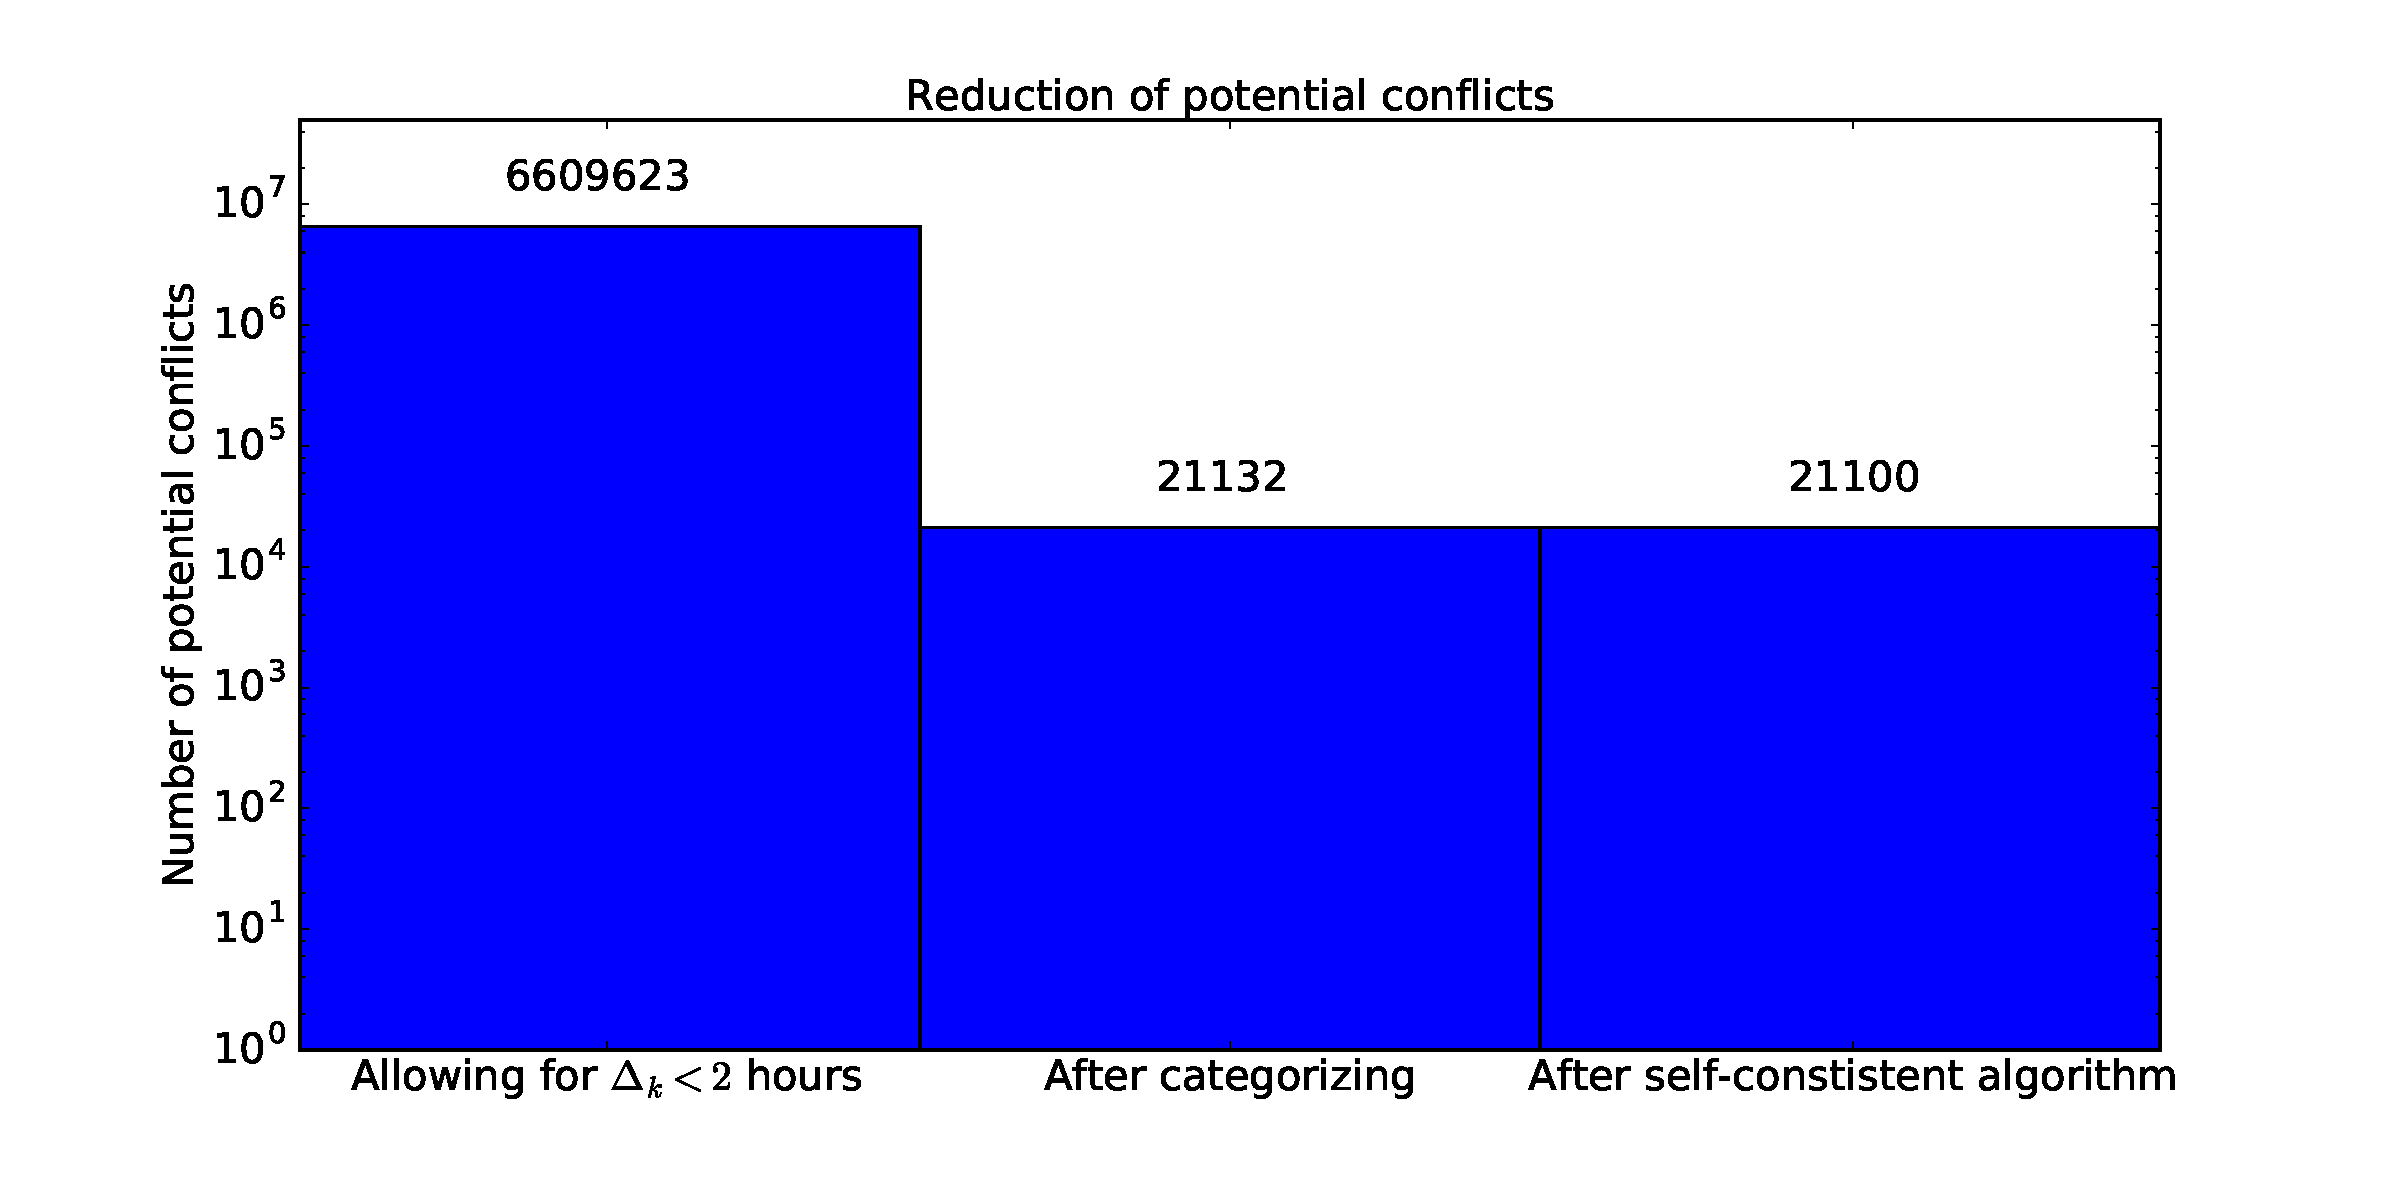
\includegraphics[width=1.0\textwidth]{images/potential_conflict_reduction.pdf}
    \end{center}
\end{frame}
\end{document}

